Die  Projektgruppe besteht  aus sieben  Teammitgliedern. Zur Erreichung  einer
effizienten Arbeitsweise ist das  Team hierarchisch organisiert. Die einzelnen
Funktionen  und  Aufgaben  der  jeweiligen Personen  sind  im  Organigramm  in
Abbildung \ref{fig:organigramm} ersichtlich. Zudem ist das Organigramm mit den
Fach-Coaches und dem Auftraggeber erg\"anzt.

%\vspace{-17mm}
%{\centering
%    %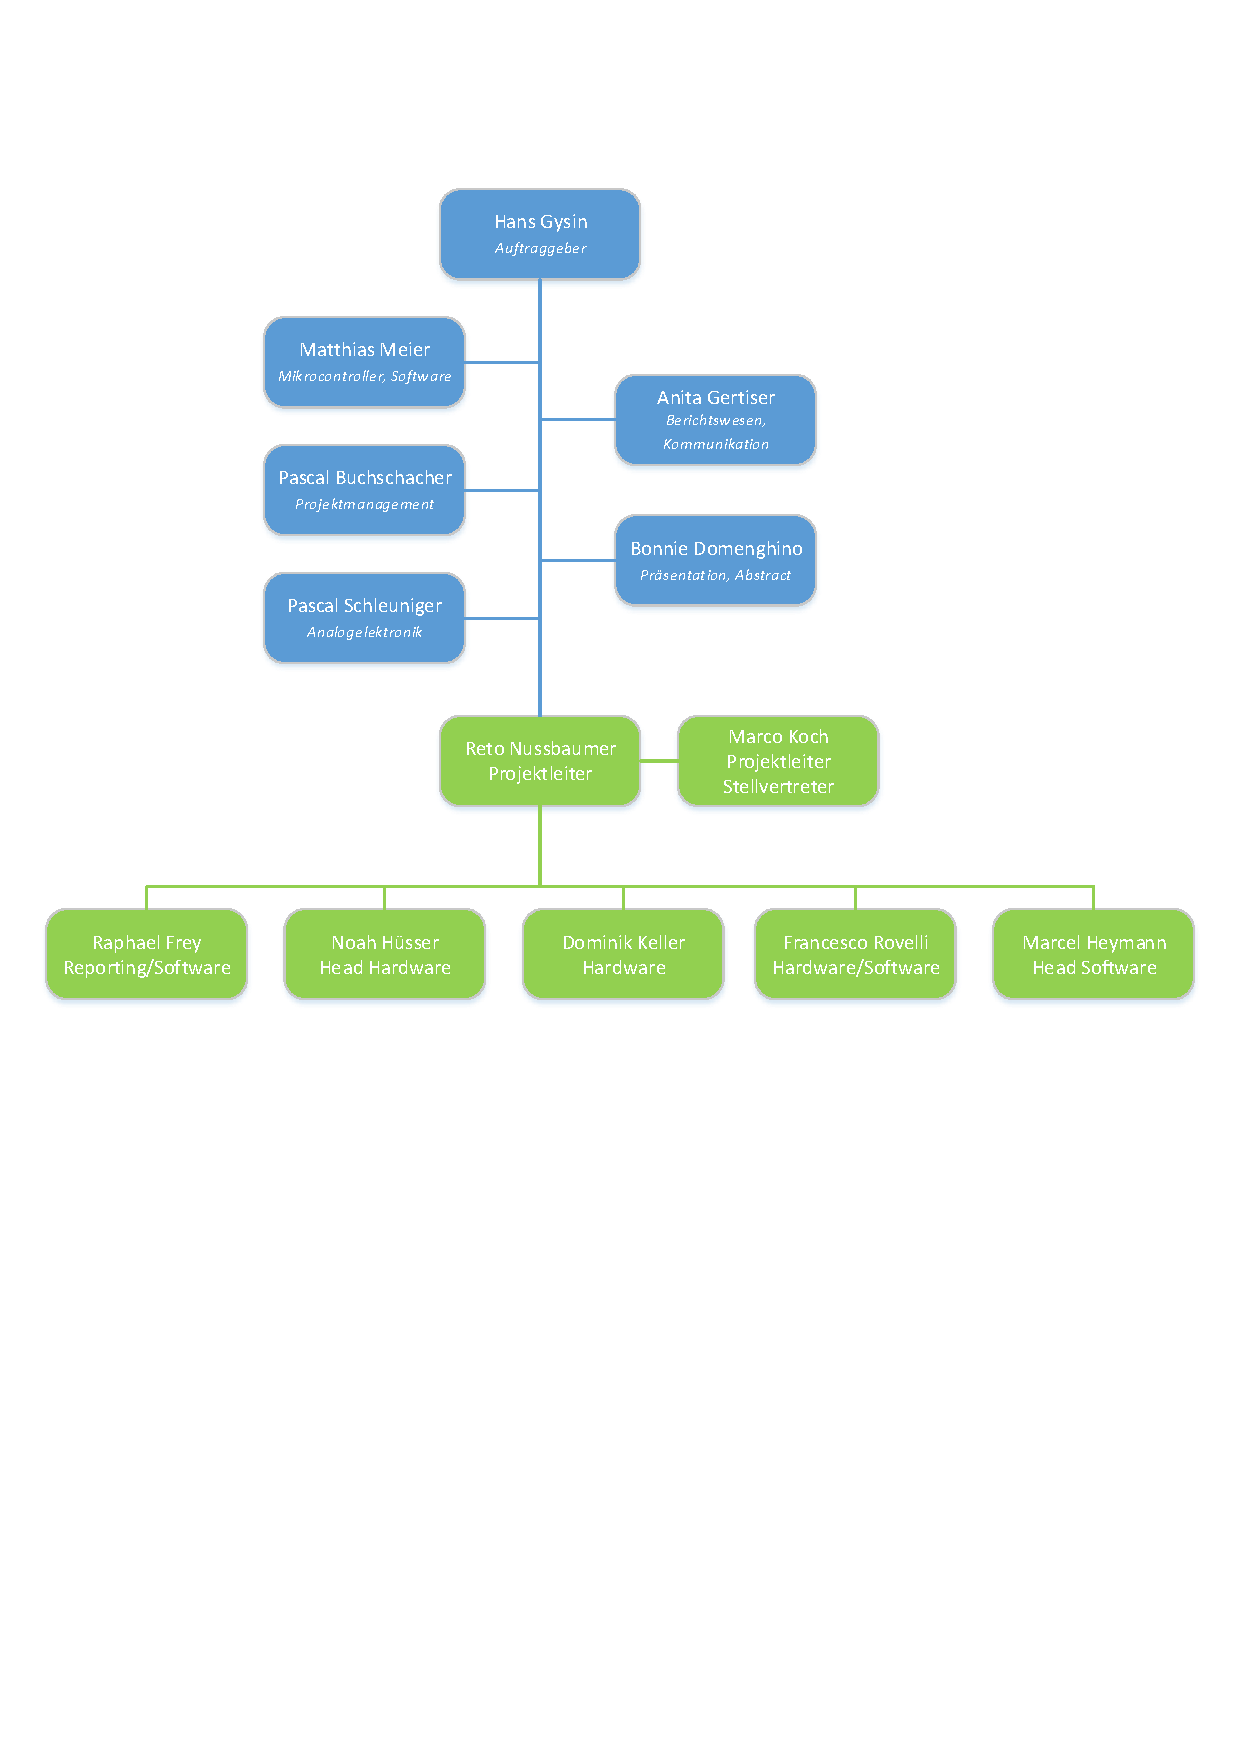
\includegraphics[width=210mm,clip=true,trim=0mm 45mm 0mm 10mm]{images/organigramm.pdf} \\
%    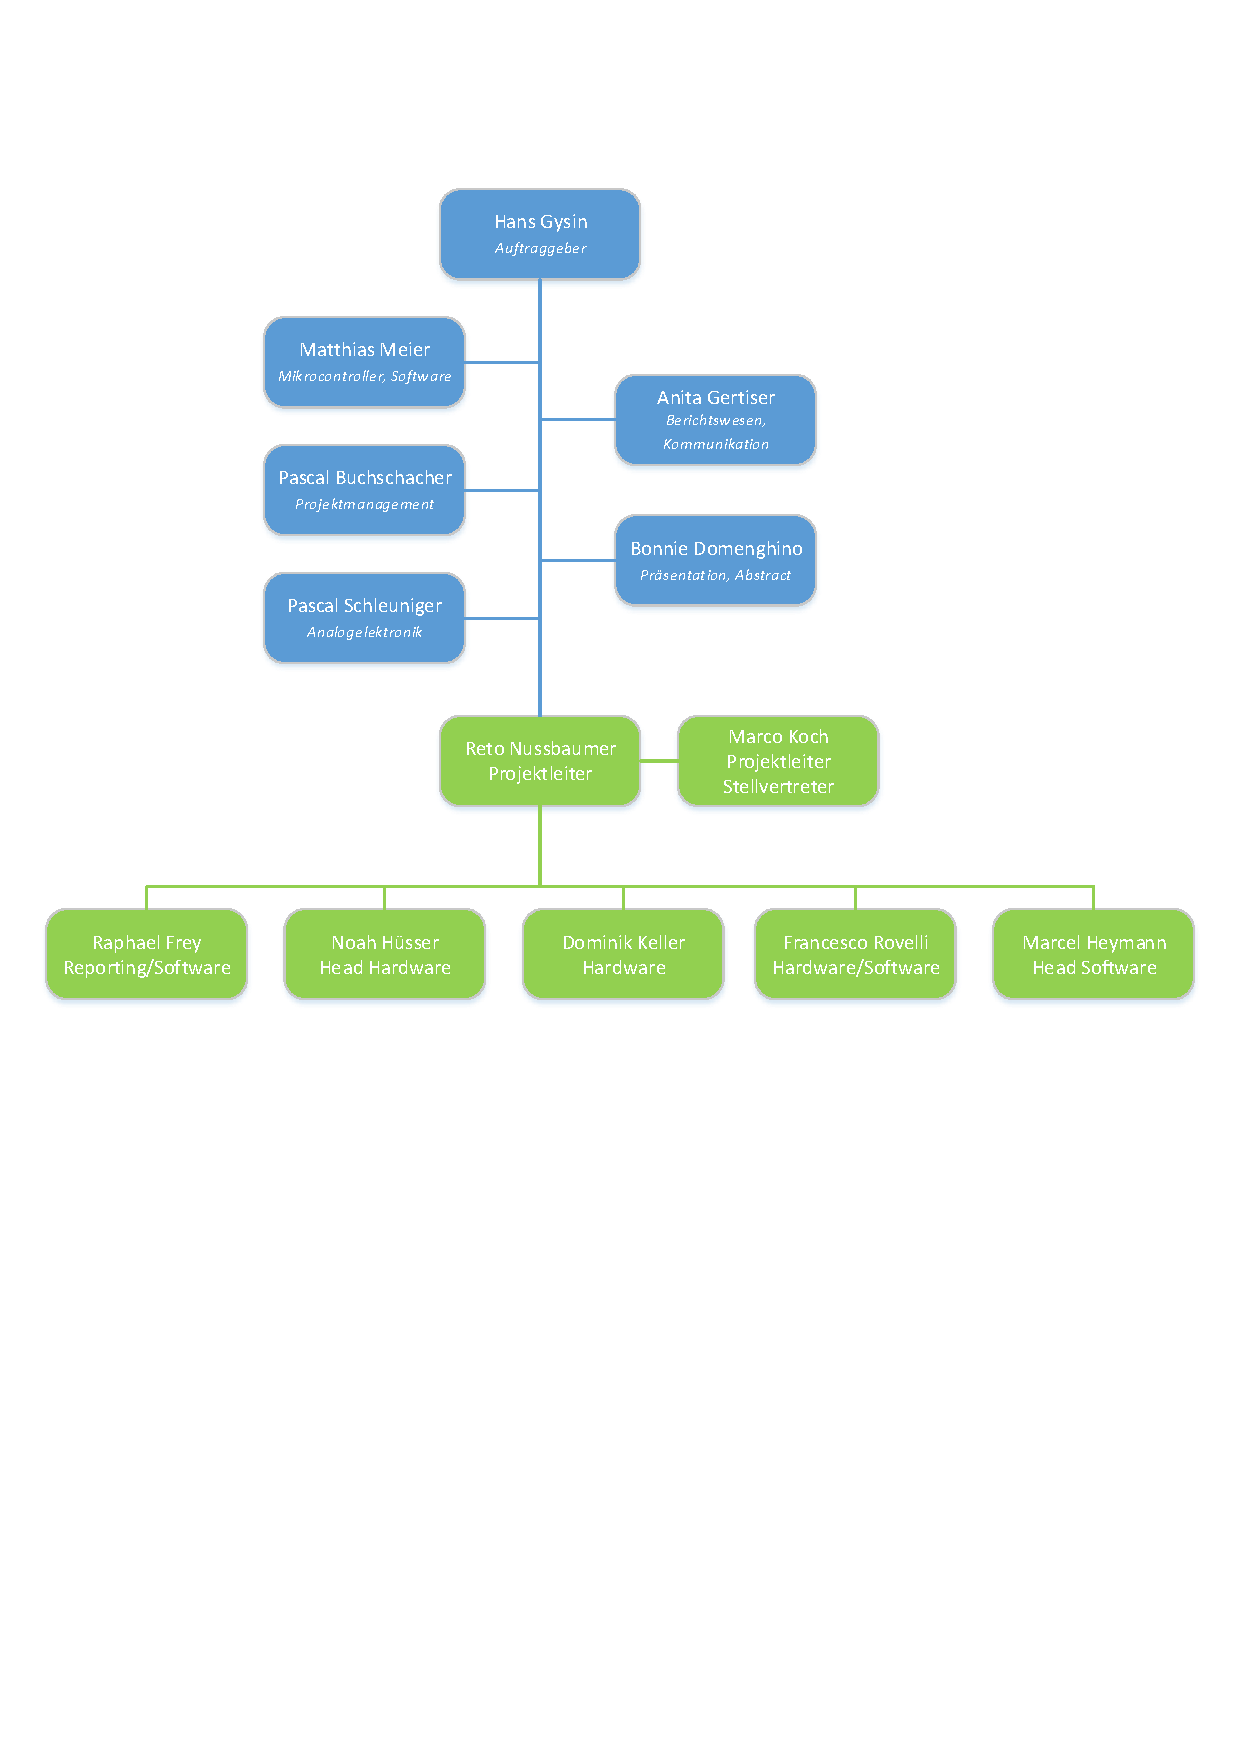
\includegraphics[width=175mm,clip=true,trim=0mm 125mm 0mm 10mm]{images/organigramm.pdf} \\
%    \label{fig:organigramm}
%    %\vspace*{-30mm}
%    \captionof{figure}{Organisationsstruktur}
%}

{\centering
    %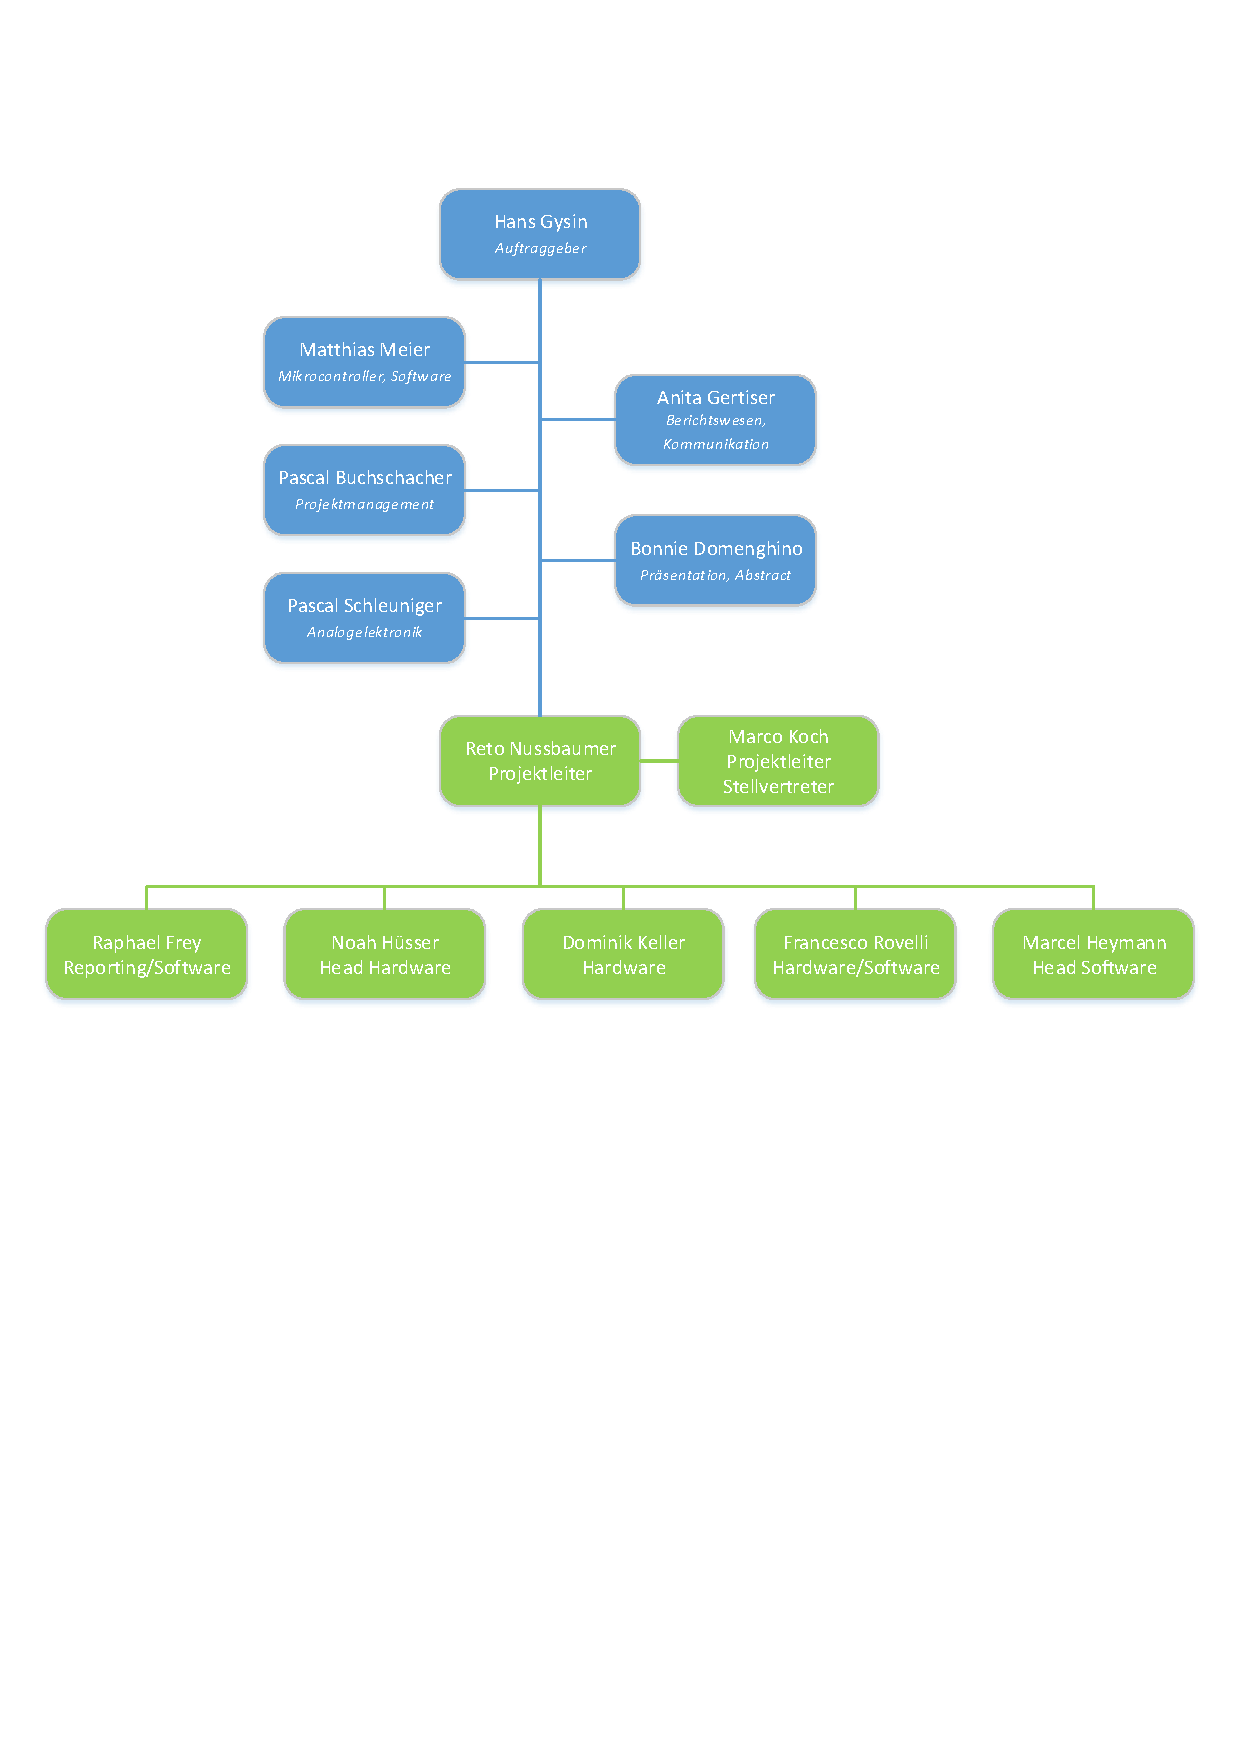
\includegraphics[width=210mm,clip=true,trim=0mm 45mm 0mm 10mm]{images/organigramm.pdf} \\
    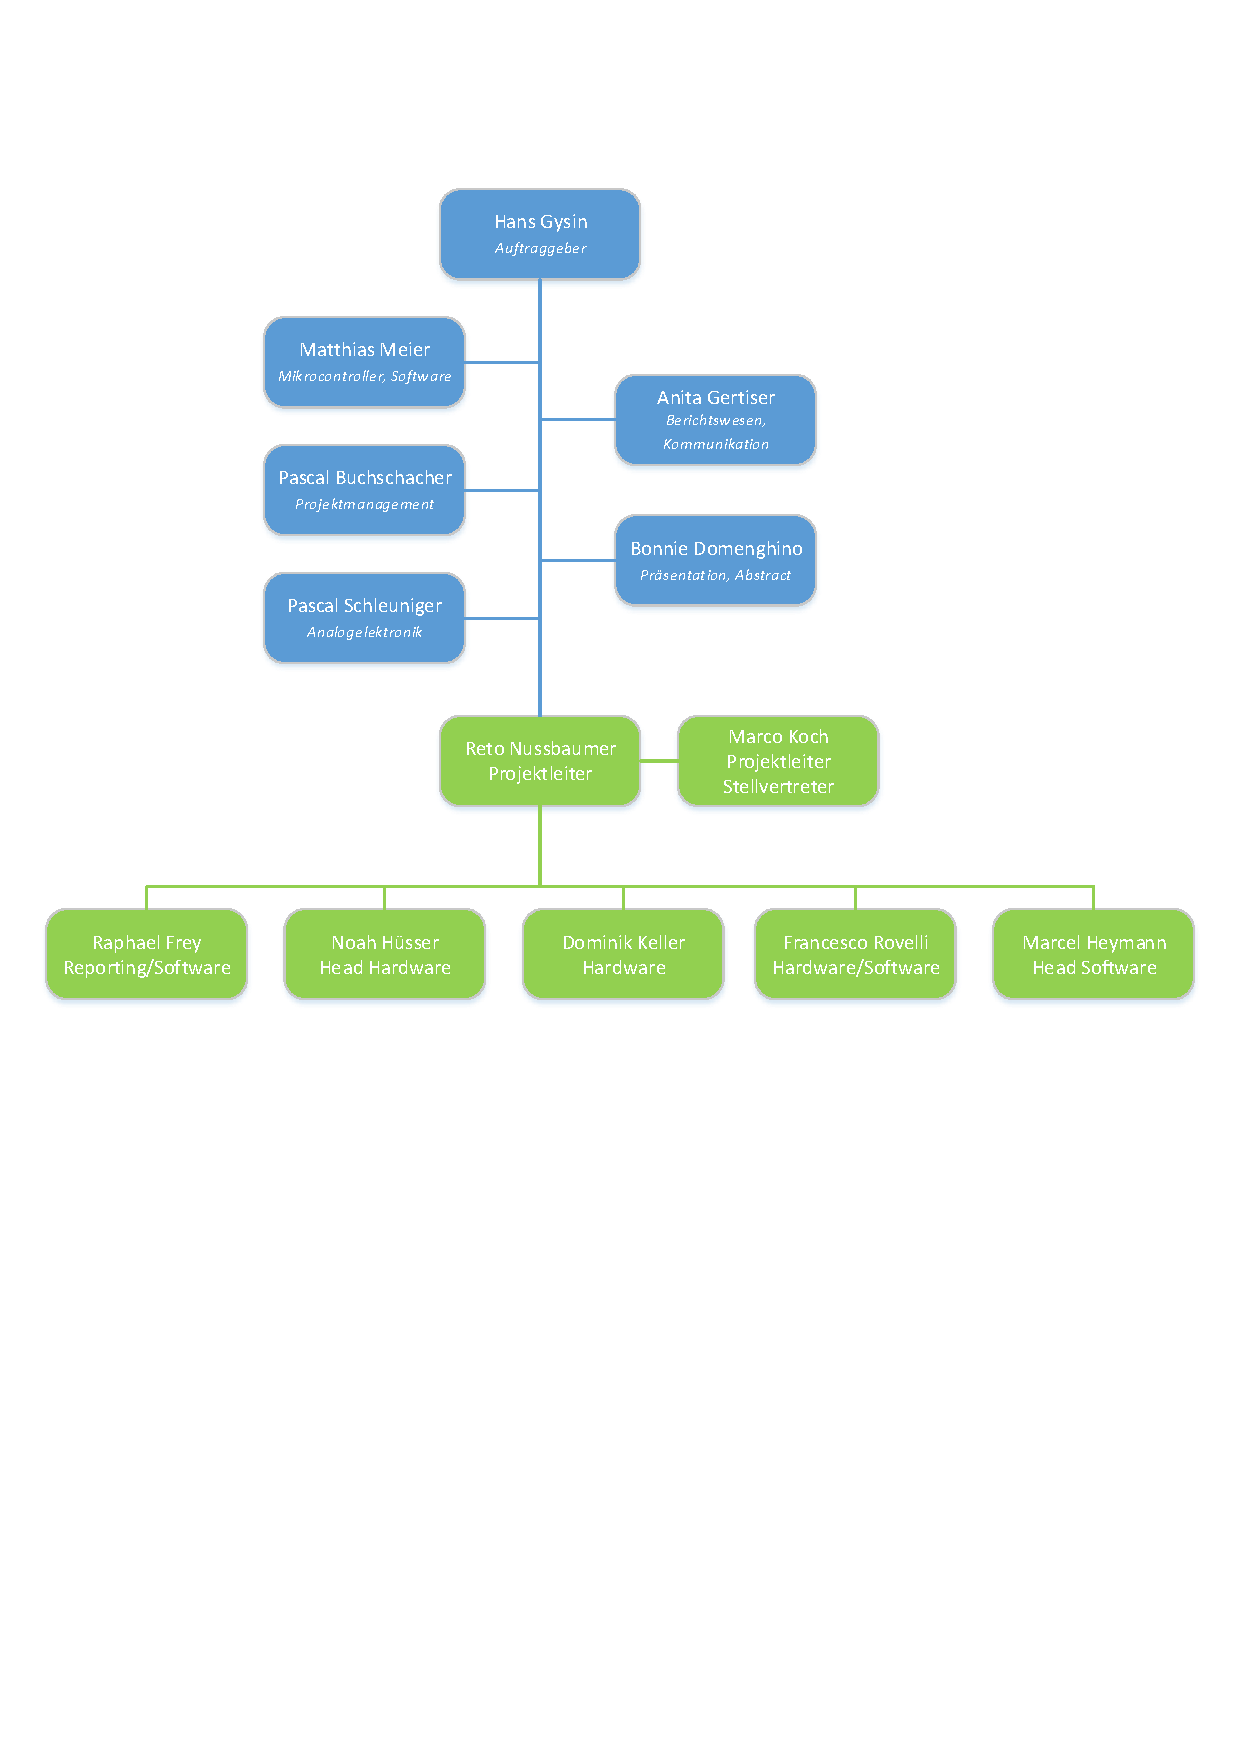
\includegraphics[width=175mm,clip=true,trim=0mm 125mm 0mm 10mm]{images/organigramm.pdf} \\
    \label{fig:organigramm}
    %\vspace*{-30mm}
    \captionof{figure}{Organisationsstruktur}
}
